
\documentclass[10pt]{article}
\usepackage{bbding}
\let\bbdSquare\Square
\let\Square\undefined
\usepackage{amsmath, amssymb}
\usepackage{graphicx}
\usepackage{epsdice}
\usepackage{physics}
\usepackage{siunitx}
\usepackage[version=4]{mhchem}
\usepackage[utf8x]{inputenc}
\usepackage{pifont}
\usepackage{xcolor}
\usepackage{listings}
\usepackage{wasysym}
\usepackage{tikz}
\usetikzlibrary{calc}
\usepackage[clock,weather,misc]{ifsym}
\usepackage{fontspec}
%\usepackage{unicode-math}
\usepackage[compat=1.0.0]{tikz-feynman}
\usepackage{chemfig}
\usepackage{verbatim}
\usepackage{skak}
\usepackage{phaistos}
\usepackage{cancel}
\usepackage{wasysym}
\usepackage{pifont}
\usetikzlibrary{matrix}


\usepackage{pgfplots}
\usepackage{pgf-pie}
\usepackage{mathtools}
\usetikzlibrary{arrows}
\usepackage{chessfss}

\usepackage{etoolbox}
\newtoggle{showpct}
\makeatletter
\patchcmd{\pgfpie@slice}%
{\scalefont{#3}\beforenumber#3\afternumber}%
{\iftoggle{showpct}{\scalefont{#3}\beforenumber#3\afternumber}{}}%
{}{}
\makeatother

\usepackage{polyglossia}
\setdefaultlanguage{english}
\setotherlanguage{korean}

\defaultfontfeatures{Scale = MatchUppercase}
\newfontfamily\koreanfont{Noto Serif CJK KR}[Script = Hangul, Language = Korean]
\newfontfamily\koreanfontsf{Noto Sans CJK KR}[Script = Hangul, Language = Korean]


\tikzset{
  treenode/.style = {align=center, inner sep=0pt, text centered,
    font=\sffamily},
  arn_n/.style = {treenode, circle, black, draw=black,
    fill=white, text width=1.5em},% arbre rouge noir, noeud noir
}


\def\slant#1#2{%
  \tikz[baseline=(X.base), xslant=tan(#1)]
    \node[inner sep=0pt, xslant=tan(#1)](X){#2};%
}

\makeatletter
\newsavebox\myboxA
\newsavebox\myboxB
\newlength\mylenA

\newcommand*\xoverline[2][0.75]{%
    \sbox{\myboxA}{$\m@th#2$}%
    \setbox\myboxB\null% Phantom box
    \ht\myboxB=\ht\myboxA%
    \dp\myboxB=\dp\myboxA%
    \wd\myboxB=#1\wd\myboxA% Scale phantom
    \sbox\myboxB{$\m@th\overline{\copy\myboxB}$}%  Overlined phantom
    \setlength\mylenA{\the\wd\myboxA}%   calc width diff
    \addtolength\mylenA{-\the\wd\myboxB}%
    \ifdim\wd\myboxB<\wd\myboxA%
       \rlap{\hskip 0.5\mylenA\usebox\myboxB}{\usebox\myboxA}%
    \else
        \hskip -0.5\mylenA\rlap{\usebox\myboxA}{\hskip 0.5\mylenA\usebox\myboxB}%
    \fi}


\newcommand\strictCeil[1]{\left|\!\xoverline[1.1]{#1}\!\right|}

%\def\molecule#1#2#3#4#5#6#7{
% \begin{scope}[shift={#1},rotate=#2]
%    \draw [fill=black] (0,0) circle (.08);
%    \draw (-0.1,0) -- ({-0.1-#3},0);
%    \draw ({-0.16-#3},0) circle (.08);
%   \draw ({0.1*cos(#6)},{-0.1*sin(#6)}) -- ({(0.1+#4)*cos(#6)},{-%(0.1+#4)*sin(#6)});
%   \draw ({(0.16+#4)*cos(#6)},{-(0.16+#4)*sin(#6)}) circle (.08);
%   \draw ({0.1*cos(#7)},{0.1*sin(#7)}) --({(0.1+#5)*cos(#7)},%{(0.1+#5)*sin(#7)});
   
 \def\moleculedos#1#2#3#4#5#6#7#8{
  \begin{scope}[shift={#1},rotate=#2]
    \draw (0,0) -- ({#3},0);
   \draw ({#3+0.1*cos(#6)},{-0.1*sin(#6)}) -- ({#3+(0.1+#4)*cos(#6)},{-(0.1+#4)*sin(#6)});
   %\draw ({0.1+#3+(0.2+#4)*cos(#6)},{-(0.2+#4)*sin(#6)}) circle (.1);
   \draw ({#3+0.1*cos(#7)},{0.1*sin(#7)}) --({#3+(0.1+#5)*cos(#7)},{(0.1+#5)*sin(#7)});
   %\draw ({0.1+#3+(0.2+#5)*cos(#7)},{(0.2+#5)*sin(#7)}) circle (.1);
   	\coordinate (3#8) at ({#3+(0.1+#5)*cos(#7)},{(0.1+#5)*sin(#7)});
   	   	\coordinate (2#8) at ({#3+(0.1+#4)*cos(#6)},{-(0.1+#4)*sin(#6)});
		\coordinate (1#8) at (0,0);
		    \draw[fill=white] ({+#3},0) circle (.1);

\end{scope}
}
\def\moleculetres#1#2#3#4#5#6#7#8{
  \begin{scope}[shift={#1},rotate=#2]
   \draw ({#3+0.1*cos(#6)},{-0.1*sin(#6)}) -- ({#3+(0.1+#4)*cos(#6)},{-(0.1+#4)*sin(#6)});
   %\draw ({0.1+#3+(0.2+#4)*cos(#6)},{-(0.2+#4)*sin(#6)}) circle (.1);
   \draw ({#3+0.1*cos(#7)},{0.1*sin(#7)}) --({#3+(0.1+#5)*cos(#7)},{(0.1+#5)*sin(#7)});
   %\draw ({0.1+#3+(0.2+#5)*cos(#7)},{(0.2+#5)*sin(#7)}) circle (.1);
   	\coordinate (3#8) at ({#3+(0.1+#5)*cos(#7)},{(0.1+#5)*sin(#7)});
   	   	\coordinate (2#8) at ({#3+(0.1+#4)*cos(#6)},{-(0.1+#4)*sin(#6)});
		\coordinate (1#8) at (0,0);
		    \draw[fill=white] ({+#3},0) circle (.1);

\end{scope}
}



\def\rotatechartwo#1{\reflectbox{#1}}

\definecolor{hanpurple}{rgb}{0.32, 0.09, 0.98}

%\newcommand{\knightB}[1][1.85ex]{%
%\adjustbox{Trim=3.2pt 2.2pt 3.2pt 0pt, width=#1, raise =-0.03ex,margin=0.14ex 0ex 0.14ex 0ex}{\BlackKnightOnWhite}%
%}

\def\slant#1#2{%
  \tikz[baseline=(X.base), xslant=tan(#1)]
    \node[inner sep=0pt, xslant=tan(#1)](X){#2};%
}


\begin{document}

	156) Song [3]
	\begin{figure}[htbp!]
		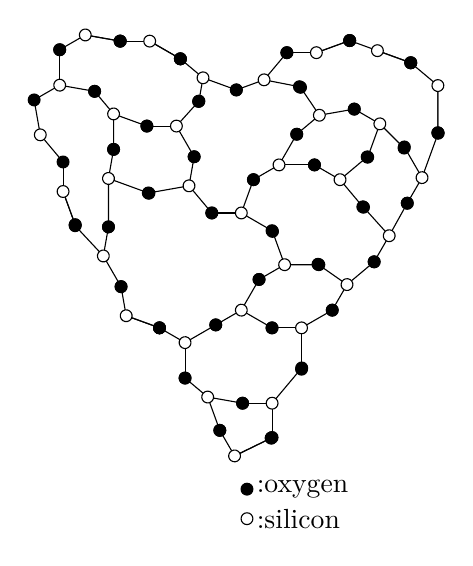
\begin{tikzpicture}[scale=.75]
		%\begin{scope}
		% \draw[]  (4,1) ..controls +(120:2cm)
        %and +(90:2cm) .. (0,0) .. controls  +(-90:2cm) and +(90:3cm) ..
        %(4,-8) .. controls +(90:3cm) and +(-90:2cm) ..(8,0)  .. controls
        %+(90:2cm) and  +(60:2cm) .. (4,1);
		%\end{scope}
      \moleculetres{(0,0)}{0}{0.5}{0.5}{0.5}{50}{100}{a}
	    \moleculedos{(3a)}{30}{0.5}{0.5}{0.5}{40}{60}{b}
		\moleculedos{(2a)}{-90}{0.5}{0.5}{0.5}{-20}{20}{i}
		\moleculedos{(3b)}{30}{0.5}{0.5}{0.5}{40}{-40}{c}
		\moleculedos{(2b)}{-50}{0.5}{0.5}{0.5}{40}{30}{d}
		\moleculedos{(2d)}{-100}{0.5}{0.72}{0.63}{-10}{80}{e}
		\moleculedos{(3d)}{0}{0.5}{0.5}{0.46}{60}{48}{f}
		\moleculedos{(2c)}{0}{0.5}{0.5}{0.5}{30}{-30}{g}
		\moleculedos{(2g)}{-40}{0.5}{0.3}{0.5}{60}{20}{h}
		\moleculedos{(2e)}{-100}{0.5}{0.6}{0.5}{127}{40}{j}
	\moleculedos{(3j)}{-80}{0.5}{0.5}{0.5}{-60}{60}{k}
		\moleculedos{(2f)}{-100}{0.5}{0.6}{0.5}{70}{50}{l}
		\moleculedos{(3k)}{-30}{0.5}{0.5}{0.5}{60}{60}{m}
		\moleculedos{(3l)}{0}{0.5}{0.5}{0.5}{30}{70}{n}
		\moleculedos{(3h)}{20}{0.5}{0.51}{0.5}{31}{30}{o}
		\moleculedos{(2m)}{-40}{0.5}{0.5}{0.5}{30}{30}{p}
		\moleculedos{(3m)}{30}{0.5}{0.5}{0.5}{60}{30}{q}				      
		\moleculedos{(3p)}{0}{0.5}{0.48}{0.68}{90}{50}{r}	
		\moleculedos{(2q)}{0}{0.5}{0.6}{0.5}{90}{30}{s}	
		\moleculedos{(3q)}{30}{0.5}{0.48}{0.5}{30}{80}{t}	
		\moleculedos{(3n)}{30}{0.5}{0.5}{0.5}{30}{30}{u}
		\moleculedos{(2u)}{-30}{0.5}{0.5}{0.5}{20}{70}{w}
		\moleculedos{(3u)}{40}{0.5}{0.5}{0.47}{30}{84}{x}
		\moleculedos{(2p)}{-60}{0.5}{0.59}{0.59}{-86}{86}{y}
		\moleculedos{(2x)}{-30}{0.5}{0.5}{0.48}{80}{-15}{z}	
		\moleculedos{(3s)}{60}{0.5}{0.5}{0.5}{20}{85}{aa}	
		\moleculedos{(3o)}{0}{0.5}{0.5}{0.5}{-20}{20}{ab}		      
	     \moleculedos{(2aa)}{60}{0.51}{0.53}{0.55}{-1}{72}{ac}		    
	     \moleculedos{(3ab)}{-20}{0.5}{0.5}{0.5}{0}{0}{ad}  
	     \moleculedos{(2ac)}{60}{0.5}{0.7}{0.5}{-10}{60}{ae}
	     \moleculedos{(2ad)}{-40}{0.6}{0.7}{0.7}{50}{-50}{af}
 
      \foreach \letter in {b,c,d,e,f,g,h,i,j,k,l,m,n,o,p,q,r,s,t,u,w,x,y,z,aa,ab,ac,ad,ae,af}{
      	\draw[fill=black] (1\letter) circle (0.1);
		\draw[fill=black] (2\letter) circle (0.1);
		\draw[fill=black] (3\letter) circle (0.1);
      }
      
      \draw[fill= black] (4,-6) circle(.1) node[right] {:oxygen};
		 \draw[] (4,-6.5) circle(.1) node[right] {:silicon};
      
      
          \end{tikzpicture}	
	\end{figure}
	
	
	157) Song [4]
	\[
		\text{\tiny a} - \text{chat}
	\]
	
	158) Book [4]
	\[
		\forall \mars \text{ such that } \mars \in \king
	\]
	
	159) Song [3]
	\[
		R_{\odot} < \frac{2GM_{\odot}}{c^2}
	\]
	
	160) Song [7]
	\[
	\schemestart
	\chemfig{HeD} 
	\arrow{-/>}
	\chemfig{u} 
	\chemfig{+} 
	\chemfig{HeHdd}
	\schemestop
	\]
	
	161) Song [8]
	\[
		\exists \gamma \text{ where } r_{\gamma} < \frac{2GM}{c^2}
	\]
	
	162) Series/Book [3,4]
	
	\begin{figure}[htbp!]
	\centering
		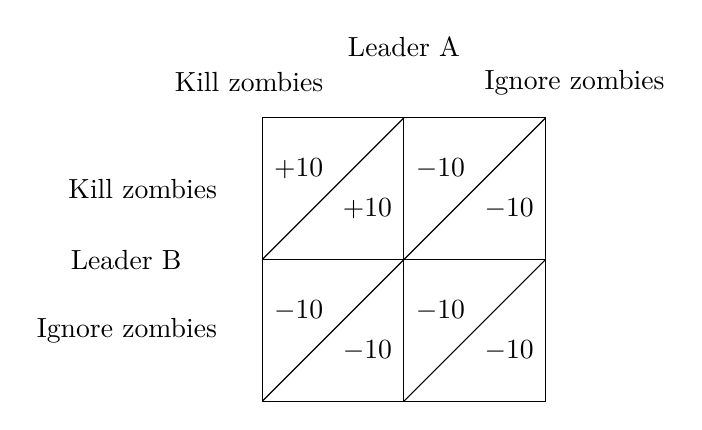
\begin{tikzpicture}[scale=0.9]
			\draw (0,0) -- (4,0) -- (4,4) -- (0,4) -- cycle;
			\draw (2,0) -- (2,4);
			\draw(0,2) -- (4,2);
			\node at (2,5) {Leader A};
			\node[left] at (-1,2) {Leader B};
			\node[left] at (1,4.5) {Kill zombies};
			\node[right] at (3,4.5) {Ignore zombies};
			\node[left] at (-0.5,3) {Kill zombies};
			\node[left] at (-0.5,1) {Ignore zombies};
			\draw (0,0) -- (2,2);
				\draw (2,0) -- (4,2);
				\draw (0,2) -- (2,4);
				\draw (2,2) -- (4,4);
			\node[above left] at(1,3) {$+10$};
			\node[below right]at (1,3) {$+10$};
			\node[above left] at(1,1) {$-10$};
			\node[below right] at(1,1) {$-10$};
			\node[above left]at (3,3) {$-10$};
			\node[below right] at(3,3) {$-10$};
			\node[above left] at(3,1) {$-10$};
			\node[below right] at (3,1) {$-10$};
		\end{tikzpicture}
	\end{figure}
	
	163) Film  [5]
	
	\texttt{try\{ }
	
	\texttt{\quad if(ucan)} 
	
	\texttt{\quad \quad throw new Exception();}
	
	\texttt{\};}
	
	\texttt{catch(Exception  i)\{}
	
	\texttt{\quad \ldots}	
	\\
	164) Song [4]
	\begin{figure}[htbp!]
		\begin{tikzpicture}
			\begin{axis}			
				[ylabel={energy},
				xlabel={$x$},
				yticklabels={,,},
				xticklabels={,,},
				axis x line = bottom,
				axis y line = left,
				ticks=none,
				title=BRaIN,
				]
				\addplot[domain=0.95:2,
						samples=200]{ (1/x)^(12) -(1/x)^6} node[above left] {$M\Pi R$};
			\end{axis}
		\end{tikzpicture}
	\end{figure}
	
	165) Series [3]
	\begin{figure}[htbp!]
		\begin{tikzpicture}
		
		\begin{scope}[xshift=-85, yshift=280,y=0.80pt, x=0.80pt, yscale=-10, xscale=10, inner sep=0pt, outer sep=0pt]
  \path[draw=black,line join=miter,line cap=butt,even odd rule,line width=0.056pt]
    %(50.9122,35.4077) .. controls (51.1450,35.1749) and (47.8866,35.1749) ..
    (47.0720,34.9422) .. controls (46.2574,34.7094) and (44.5119,34.1276) ..
    (44.5119,34.1276) .. controls (44.5119,34.1276) and (39.1006,32.2657) ..
    (38.4606,29.6473) .. controls (37.8205,27.0290) and (38.3442,29.2982) ..
    (37.5296,26.9126) .. controls (37.0421,25.4809) and (36.8463,25.3757) ..
    (35.9004,23.5960) .. controls (35.9004,22.0250) and (31.8856,23.8288) ..
    (30.9546,24.7597) .. controls (30.0237,25.6907) and (29.7909,27.7272) ..
    (29.6164,29.8800) .. controls (29.4418,32.0329) and (29.1509,32.6148) ..
    (28.8018,33.0802) .. controls (28.4527,33.5457) and (27.2308,34.0112) ..
    (25.2525,34.4185) .. controls (23.2742,34.8258) and (22.8087,35.0586) ..
    (22.1686,34.6513) .. controls (21.5286,34.2440) and (20.1322,33.2548) ..
    (18.5612,33.1966) .. controls (15.6953,33.4942) and (14.2941,34.7255) ..
    (11.4043,34.9422); .. controls (10.5316,35.0004)and (9.0769,35.0004) ..  
    (9.0769,35.0004);
    \end{scope}
    
    \draw[->] (0,0) -- (11,0) node[right] {frequency}; 
    \draw[->] (0,0) -- (0,5) node[above] {wavenumber};  
    \draw[->] (5,3.7) node[above] {\ce{HArRe}} -- (6,3.2);
	\draw[->] (8,4) node[above] {\ce{WILiAm}} -- (7,3.5);
    \end{tikzpicture}

	\end{figure}
	
	166) Film [4]
	\[
	\dfrac{2\bcancel{t}\epsdice{3}}{\bcancel{t}}
	\]
	
	167) Film [2]
	{\DeclareFontFamily{U}{dice3d}{}
\DeclareFontShape{U}{dice3d}{m}{n}{<-> s*[4] dice3d}{}
	\begin{figure}[htpb!]
	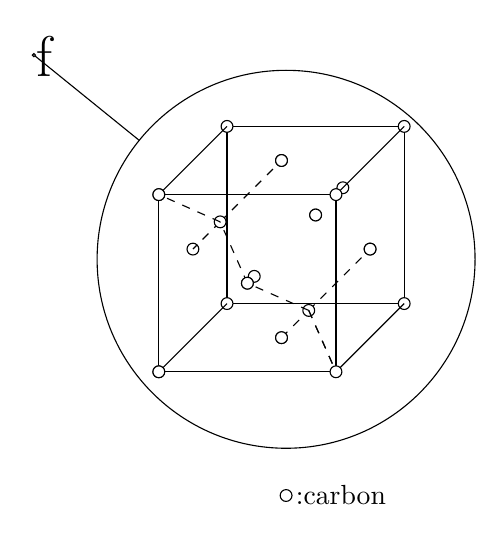
\begin{tikzpicture}
	
	
	\node at (140:4) {\huge \Pisymbol{dice3d}{102}
};
	\draw (0,0) circle (2.4); 
	\draw (141:2.4) -- (141:4.1);
	\draw (141:4.12)  circle (0.02);
\begin{scope}[scale=0.75,xshift=-1cm,yshift=-0.75cm]
\draw[fill=white] (3/2,0,3/2) circle (0.1);
\draw[dashed] (3/2,0,3/2) -- (3/2+3/4,3/4,3/2+3/4);

\draw[dashed]  (3/2+3/4,3/4,3/2+3/4) -- (3,3/2,3/2);
\draw[fill=white] (3/2+3/4,3/4,3/2+3/4) circle (0.1);



\draw[dashed] (3/2+3/4,3/4,3/2+3/4) -- (3,0,3);
\draw[dashed] (3/2+3/4,3/4,3/2+3/4) -- (3/2,3/2,3);
\draw[dashed] (3/2+3/4,3/4,3/2+3/4) -- (3,0,3);



\draw[fill=white] (3/4,3/4,3/4) circle (0.1);
\draw[fill=white] (3/2+3/4,3/4+3/2,3/4) circle (0.1);

\draw[fill=white] (0,3/2,3/2) circle (0.1);
\draw[dashed] (3/4,3/4+3/2,3/4+3/2) -- (0,3/2,3/2);

\draw[dashed] (3/4,3/4+3/2,3/4+3/2) -- (3/2,3,3/2);


\draw[fill=white] (3/4,3/4+3/2,3/4+3/2) circle (0.1);
\draw[dashed] (3/4,3/4+3/2,3/4+3/2) -- (0,3,3);



\draw[dashed] (3/2,3/2,3) -- (3/4,3/4+3/2,3/2+3/4);

\draw[fill=white] (3/2,0,3/2) circle (0.1);
\draw[fill=white] (3/2,3/2,0) circle (0.1);
\draw[fill=white] (3,3/2,3/2) circle (0.1);
\draw[fill=white] (3/2,3,3/2) circle (0.1);
\draw[fill=white] (3/2,3/2,3) circle (0.1);


\draw[] (0,0) -- (3,0) -- (3,3) -- (0,3) -- cycle;

\foreach \x in{0,3}{
	\foreach \y in{0,3}{
		\draw[fill=white] (\x,\y) circle (0.1);
	}
}

\foreach \x in{0,3}{
	\foreach \y in{0,3}{
		\draw[] (\x,\y,0) -- (\x,\y,3);
	}
}


\draw[] (0,0,3) -- (3,0,3) -- (3,3,3) -- (0,3,3) --(0,3,3) -- cycle;

\draw[fill=white] (0,0,3) circle (0.1);
\draw[fill=white] (0,3,3) circle (0.1);




\foreach \x in{0,3}{
	\foreach \y in{0,3}{
		\draw[fill=white] (\x,\y,3) circle (0.1);
	}
}
\draw[fill=white] (3/2,3/2,0) circle (0.1);
\draw[fill=white] (3,3/2,3/2) circle (0.1);
\draw[fill=white] (3/2,3,3/2) circle (0.1);
\draw[fill=white] (3/2,3/2,3) circle (0.1);

\end{scope}

\draw( 0,-3) circle (0.075) node[right] (0,-3) {:carbon};

\end{tikzpicture}
\end{figure}
}
	
	168) Film [7]
	
	\begin{figure}[htbp!]
	\begin{tikzpicture}
	\draw[<->] (0,0.5) node[above] {N} -- (0,-0.5)node[below] {S};
	\draw[<->] (-0.5,0) node[left] {W}-- (0.5,0) node[right] {E};
	\draw[fill=black] (-2.4,0) circle (0.02) node[above] {$\frac{1}{t}$};
	\draw[fill=black] (-3,0) circle (0.02) node[above] {$\frac{1}{t}$};
		\draw[fill=black] (-3.2,0) circle (0.02) node[above] {$\frac{1}{t}$};
	\end{tikzpicture}
	\end{figure}
	
	169) Film [2]
	\[
	\schemestart
	\chemup.
	\chemfig{Me-NT}
	\chemdown.
	\arrow{->}
	\chembelow{
	\chemup.
	\chemfig{Me} \quad
	\chemfig{ + } \quad
	\chemfig{NT}
	\chemdown\}}{this}
	\schemestop
	\]
	
	170) Film [2]
	\[
	\schemestart
	\chemup.
	\chemfig{InTa-NUMo}
	\chemdown.
	\arrow{->}
	\chembelow{
	\chemup.
	\chemfig{InTa}\quad 
	\chemfig{ + } \quad
	\chemfig{NUMo}
	\chemdown\}}{this}
	\schemestop
	\]
	
	171) Book [3]
	\[
		f(x) = 39H(x) = \begin{cases}
			0 & x \leq 0\\
			39 & x > 0 \\
		\end{cases}
	\]
	
	
	172) Book/Film [6]
	\[
	\cfrac{H_1N_1}{\text{\PHeagle} + \cfrac{H_1N_1}{\text{\PHeagle} + \cfrac{H_1N_1}{\text{\PHeagle} + \ldots}}}
	\]
	
	173) Book/Film [2]
	\[		
		\text{Indexed family } \{(U_\alpha, \gamma_\alpha) : \alpha \in I\} \text{ of charts on \Cloud\ which covers \Cloud} 
	\]
	
	174) Game [1]
	
	\[
	|f(x)|\leq \earth \text{ for all } x
	\]
	
	175) Song [4]
	\[
	3\female
	\]
	
	176) Song [1]
	\begin{figure}[htbp!]
	\centering
		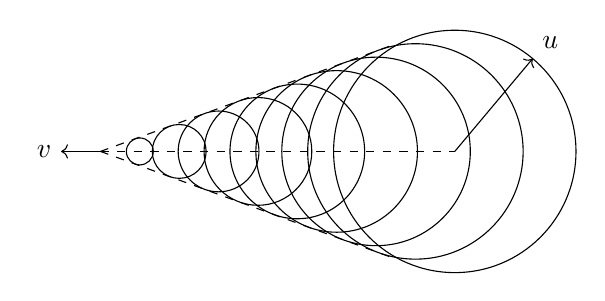
\begin{tikzpicture}
			\draw[dashed] (0,0) -- (20:4);
			\draw[dashed] (0,0) -- (-20:4);
			\foreach \i in {1,...,9} {
			\draw ({\i*0.5},0) circle ({\i*0.5*sin(20});
			}
			\draw[->] (0,0) -- (-0.5,0) node[left] {$v$};
			\draw[->] (4.5,0) -- + (50:1.53909064497) node[above right] {$u$};
			\draw[dashed] (0,0) -- (4.5,0);
		\end{tikzpicture}
	\end{figure}

	177) Album/Song [6]
	\[
	\frac{\in \text{\Plane}}{C}
	\]
	
	178) Album/Song [2]
	\begin{figure}[htbp!]
	\centering
		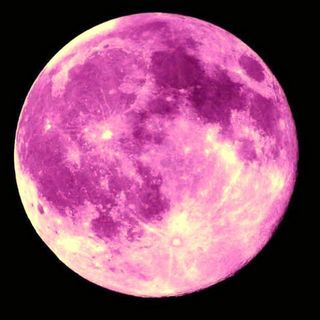
\includegraphics[scale=0.4]{./pinkmoon.jpg}
	\end{figure}
	
	179)  Song [3]
	\[
	{\color{red} e} \lor \lnot {\color{red} e}
	\]
	
	180) Song [3]
	\[
		\{a,b, c, k,l\} \setminus \{l\}
	\]
	
	181) Song [4]
	\[
		\text{me} \notin \heartsuit
	\]

	182) Song [5]
	
	\[
		\{1,1,1,1\} \in \text{life} \in \text{me}
	\]
	
	183) Song [2]
	\begin{figure}[htbp!]
		\centering
		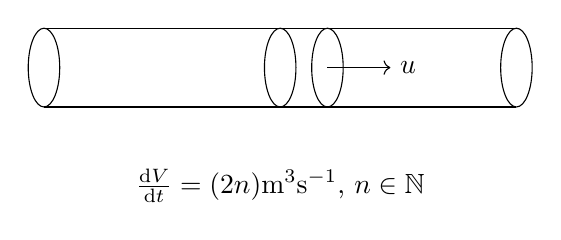
\begin{tikzpicture}[scale=2]
			\draw (0,0) -- (3,0);
			\draw (0,0.25) circle (0.1 and 0.25);
			\draw (3,0.25) circle (0.1 and 0.25);
			\draw (0,0.5) -- (3,0.5);
			\draw (1.5,0.25) circle (0.1 and 0.25);
			\draw (1.8,0.25) circle (0.1 and 0.25);
			\draw[->] (1.8, 0.25) -- (2.2,0.25) node[right] {$u$};
			\draw (1.8,0) --(2.2,0);
			\draw (1.8,0.5) -- (2.2,0.5);
			
			\node at (1.5,-0.5) {$\dv{V}{t} = (2n)\si{\metre^3 \second^{-1}}$, $n \in \mathbb{N}$}; 
		\end{tikzpicture}
	\end{figure}
	
	184) Series [1]
	\[
	\rho_m
	\]
	
	\definecolor{cff0000}{RGB}{255,0,0}
\definecolor{cffffff}{RGB}{255,255,255}


	185) Film [4]
	\begin{figure}
	\centering


\begin{tikzpicture}[y=0.80pt, x=0.80pt,rotate=37.75
, yscale=-30, xscale=30, inner sep=0pt, outer sep=0pt]

  \path[draw=black,fill=cff0000,miter limit=4.00]
    (15.0813,61.6683)arc(270.003:180.001:1.832)arc(180.003:89.997:1.832)arc(89.999:-0.003:1.832)arc(359.999:270.001:1.832)
    -- cycle;



  \path[draw=black,fill=cffffff,miter limit=4.00]
    (19.1912,63.5000) .. controls (19.1912,64.3671) and (18.4883,65.0700) ..
    (17.6212,65.0700) .. controls (17.1983,65.0700) and (16.8144,64.9027) ..
    (16.5321,64.6308) .. controls (16.5321,64.6308) and (16.5210,62.4102) ..
    (16.5356,62.3659) .. controls (16.8176,62.0959) and (17.2000,61.9300) ..
    (17.6212,61.9300) .. controls (18.4883,61.9300) and (19.1912,62.6329) ..
    (19.1912,63.5000) -- cycle;



  \path[draw=black,fill=cffffff,miter limit=4.00]
    (13.9805,59.5401) .. controls (14.8085,59.2828) and (15.6883,59.7456) ..
    (15.9456,60.5736) .. controls (16.0801,61.0068) and (16.0177,61.4541) ..
    (15.8090,61.8191) .. controls (15.8210,61.8502) and (13.5808,62.3402) ..
    (13.6485,62.3916) .. controls (13.3243,62.2005) and (13.0674,61.8928) ..
    (12.9469,61.5051) .. controls (12.6897,60.6771) and (13.1524,59.7973) ..
    (13.9805,59.5401) -- cycle;
    
      \node[below left] at (15.0812,63.5302) {\ce{O}};
      \node[right]  at (17.812,63.5302){\ce{H}};
  \draw[<->]
    (15.0812,63.5302) -- (17,63.5302) node[below right] {$0.96L$} -- (17.6212,63.5302);
    
   	\begin{scope}[shift={ (15.0812,63.5302)}]
 	\coordinate (a) at  (-52.25:1);
 	\node[above] at (a) {$104.5^{\circ}$};
 	\end{scope}
	 \draw[<->] (16,63.5302) arc (0:-104.5:1);

  \draw[->]
    (17.6212,63.5302) -- (17.8920,61.9548) node[above left] {$1.2L$\qquad };

  \draw[->]
    (15.0812,63.5302) -- (15.5501,65.2568) node[below right] {$1.4L$};
\end{tikzpicture}
	\end{figure}
	
	186) Film [1]
	\[
		f_\text{system}(t), \text{ } f_\text{subsystem}(-t)
	\]
	
	187) Album/Song [2]
	\begin{figure}[htbp!]
	\centering
    \chemfig{\vphantom{S}-[@{left,0.5}]C~S(-[6]U-[6]Re)-[@{right,0.5}]}
    \polymerdelim[height = 5pt, depth=70pt, indice = \!\!n]{left}{right}
  \end{figure}	
	
  188)Song [2]
  \begin{figure}[htbp!]
	\centering
	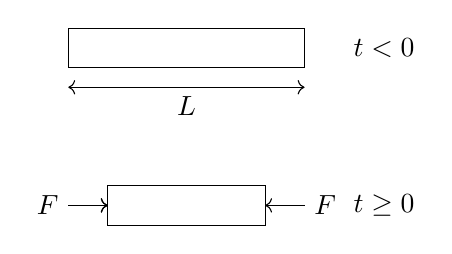
\begin{tikzpicture}
	\begin{scope}
	\draw (0,0) -- (3,0) -- (3,0.5) -- (0,0.5) -- cycle;
		\draw[<->] (0,-0.25) -- (1.5,-0.25) node[below] {$L$} -- (3,-0.25);

	\node[right] at (3.5,0.25) {$t < 0$}; 
	\end{scope}
	\begin{scope}[shift={(0.5,-2)}]
	\draw (0,0) -- (2,0) -- (2,0.5) -- (0,0.5) -- cycle;
	\draw[->] (-0.5,0.25) -- (0,0.25);
		\draw[->] (-0.5,0.25) node[left] {$F$} -- (0,0.25);
		\draw[->] (2.5,0.25) node[right] {$F$} -- (2,0.25);
		\node[right] at (3,0.25) {$t \geq 0$};
	\end{scope}
	\end{tikzpicture}
	\end{figure}


  189) Song[2] 
    \begin{figure}[htbp!]
      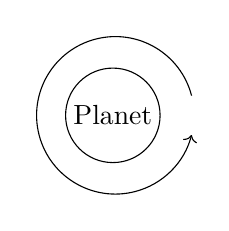
\begin{tikzpicture}
        \draw (0,0) circle (0.6) node {Planet};
        \draw[->](1,0.25) arc (14.47:360-14.47:1);
        \node at (1,-0.05) {\heartsuit};
      \end{tikzpicture}
    \end{figure}

  190) Song [2]
  \begin{figure}[htbp!]
\feynmandiagram [layered layout, horizontal=b to c] {
a -- [photon] b
-- [fermion, half left, looseness=1.5, edge label =\(\text{Insane}\)] c
-- [fermion, half left, looseness=1.5] b,
c -- [photon] d,
};

  \end{figure}

  191) Film [2]

  \[
    \underbrace{\text{Historic Data} \to \text{DAY Algorithm} \to \text{Predictive Model}}_\text{this} 
  \]
  \[
    \text{New Data} \to \text{Predictive Model} \to \text{Prediction}
  \]

  192) Film [1]
  \[
    \texttt{const een}
  \]

  193) Film [6]
  \[
  \texttt{for(\$ = n, \$ < n + m,  \$++)\{\ldots }
  \]

  194) Song [3]
  \[
    \textrm{Granite with uranium}
  \]
  
  195) Song [5]
  \[
    \{\text{\Fire}, \ldots,\text{\FilledRainCloud} \} 
  \]

  196) Film [3]
  \[
    \frac{\male}{3}
  \]

  197) Film [3]
  \[
    BR = \begin{pmatrix}
      \underbrace{\frac{1}{\sqrt{1-v^2/c^2}}}_{\text{this}} & \\
          & \ddots \\
        \end{pmatrix}
  \]

  198) Song[2] 
    \begin{figure}[htbp!]
      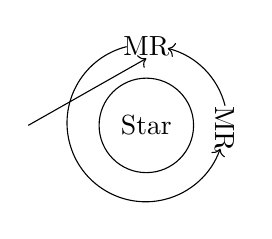
\begin{tikzpicture}
        \draw (0,0) circle (0.6) node {Star};
        \draw[->](1,0.25) arc (14.04:90-14.04:1);
        \node[rotate=-90] at (1,-0.05) {\text{MR}};
        \node at (0,1) {\text{MR}};
        \draw[->](-0.25,1) arc (90+14.04:360-19:1);
        \draw[->](-1.5,0) --(0,0.85);
      \end{tikzpicture}
    \end{figure}

\end{document}
